\documentclass[10pt]{article}
\usepackage{commands}

\begin{document}
\begin{tcolorbox}
  \begin{center}
  \begin{Large}
    \textbf{PHYS 411 (Entanglement in Many-Body Systems) Notes} \\
    \vspace{5pt}
  \end{Large}
  \begin{large}
        Rio Weil \\
\vspace{5pt}
    \emph{This document was typeset on \today}
  \end{large}
  \end{center}
\end{tcolorbox}

\begin{center}
  \textbf{Introduction:}

  This is a set of lecture notes taken from UChicago's PHYS 411 (Entanglement in Many-Body Systems), taught by Michael Levin. Topics covered include...

\end{center}
\addtocontents{toc}{\protect\hypertarget{toc}{}}
\tableofcontents

\newpage
\section{Toric Code I}

\subsection{Course Overview + Logistics}
Instructor email: \texttt{malevin@uchicago.edu}

\noindent Office: MCP 447

\noindent Evaluation: Once every $\sim 2$ weeks, 100\%.

\noindent Textbook: None; papers/references will be provided.

This class will cover topics at the interface of quantum many-body/condensed matter theory and quantum information. This has been a dynamic interface for a couple decades now, with the two fields inspiring each other. The topics chosen are both interesting from a physics point of view, but also deeply important in QI. A rough schedule is as follows:

\begin{enumerate}[(I)]
    \item \textbf{Anyons and topological quantum computation.} Anyons exist in 2-d quantum systems that have exchange statistics that are not bosonic or fermionic; the exchange phase can be anything (hence the name). Anyons first emerge in discussion of the fractional quantum hall effect, but in the last 20 years, people (lead by Alexei Kitaev) have found interesting connections between anyons and quantum computing.
    \item \textbf{Symmetry-protected topological phases.} This is another important topic in condensed matter, but is deeply connected to concepts in quantum information, e.g. finite depth-circuits (indeed they provide a quantum-information theoretic way to define phases of matter).
    \item \textbf{Entanglement entropy in many-body systems.} EE gives a lot of insight into the physics of MB systems. This also has practical applications, leading to numerical algorithms using...
    \item \textbf{Matrix product states.}
\end{enumerate}

\subsection{Defining the Toric Code Model}
References: Kitaev's lecture notes \texttt{arXiv:0904.2771}, original paper \texttt{arXiv:quant-ph/9707021}.

The toric code is an exactly solvable spin model (it can also be thought of a quantum error correcting code, but we introduce it as a spin model to start). It has:
\begin{enumerate}
    \item Anyon excitations
    \item Topological ground state degeneracy
\end{enumerate}
We consider this model on different kinds of lattices and geometries, but for now we consider the square lattice, and place a spin-1/2 degree of freedom on each of the edges of the lattice (we don't specify the boundary conditions yet). The Hilbert space has dimension $2^N$ with $N$ the total number of edges/spins. The Hamiltonian takes the following form:
\begin{equation}
    H = -\sum_s A_s - \sum_p B_p
\end{equation}
the $s$ are vertices on the lattice and $p$ are plaquettes.

\begin{center}
    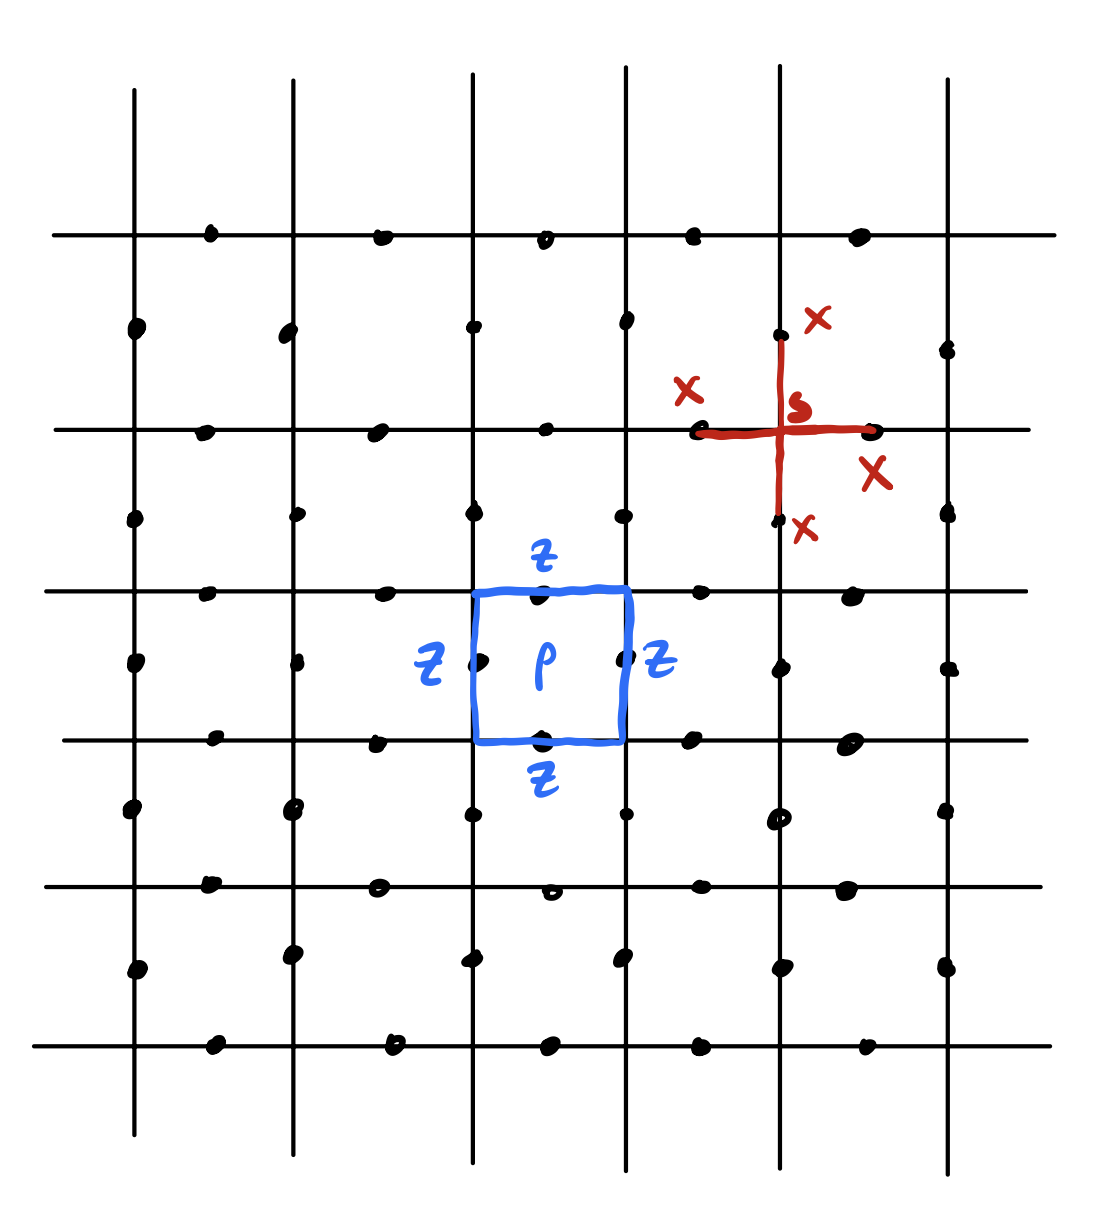
\includegraphics[scale=0.4]{Lectures/Images/lec1-toriccodeops.png}
\end{center}

The $A_s$ term is a product of Pauli-X operators on stars about vertices $s$:
\begin{equation}
    A_s = \prod_{j \in \text{star}(s)} X_j
\end{equation}
And the $B_p$ term is a product of Pauli-$Z$ operators on the boundaries of plaquettes:
\begin{equation}
    B_p = \prod_{j \in \p p}Z_j
\end{equation}
We adopt the QI notation:
\begin{equation}
    X = \sigma^x = \paulix
\end{equation}
\begin{equation}
    Y = \sigma^y = \pauliy
\end{equation}
\begin{equation}
    Z = \sigma^z = \pauliz
\end{equation}'

\subsection{Solving the toric code model}
Notice that all of the $A_s$ and $B_p$ terms commute with one another. For example, its trivial to see that:
\begin{equation}
    [A_s, A_{s'}] = [B_p, B_{p'}] = 0
\end{equation}
because $X$s are mutually commuting and $Z$s are mutually commuting. Slightly less obvious is that the star terms commute with the plaquettes:
\begin{equation}
    [A_s, B_p] = 0
\end{equation}
We might be worried if this holds because $X$ and $Z$ anticommute. But in fact the above holds; if the star and plaquette are faraway then there are no overlapping $X, Z$s so they commute. In the case where the star/plaquette overlap, we have that two $X, Z$s overlap (see picture below) so the anticommutation cancels to a commutation.

\begin{center}
    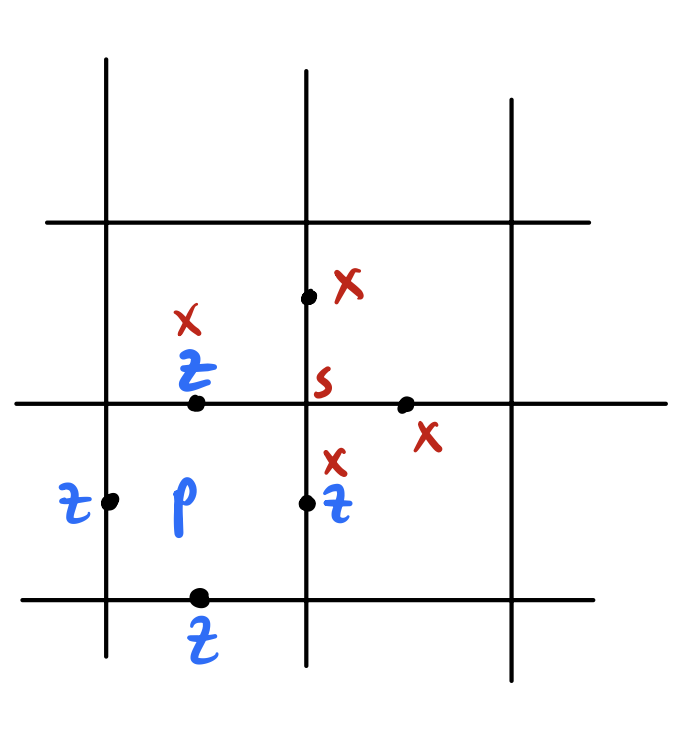
\includegraphics[scale=0.4]{Lectures/Images/lec1-toricopcommute.png}
\end{center}

Thus, we are able to simultaneously diagonalize $\set{A_s, B_p}$. Denote the eigenstates by $\ket{\set{a_s, b_p}}$ where the $a_s, b_p$ are the eigenvalues. If we have residual degeneracy, we may require additional quantum numbers to specify the state, but let us not worry about this quite yet. Note that because:
\begin{equation}
    A_s^2 = B_p^2 = \II
\end{equation}
this implies that the eigenvalues are:
\begin{equation}
    a_s, b_p = \pm 1.
\end{equation}
And the $\ket{set{a_s, b_p}}$ are also the energy eigenstates, with energy:
\begin{equation}
    E = -\sum_s a_s - \sum_p b_p.
\end{equation}
This is the sense in which the problem is exactly solvable. We have found all of the eigenstates, and can find their degeneracies by figuring out the degeneracies of $\set{a_s, b_p}$.

For the ground state, we set $a_s = b_p = 1$. We can ask the question; how many states are there that satisfy this? This is equivalent to asking what the ground state degeneracy is. The answer to this question is dependent on the geometry of the model. Let's start with the simplest, and arguably the most important case; the infinite plane. Let us work in the $X$-basis. In this basis, the different basis states are $\ket{\pm} \otimes \ket{\pm} \otimes \ldots$ for each link. A useful visualization will be in terms of strings on this lattice. In this string picture, we will say that $X_j = -1$ corresponds to a string on link $j$. On the other hand, if $X_j = +1$ then we will say that there is no string on the link. Thus, we can view an arbitrary $X$ basis state as strings occupying the lattice in some configuration.

\begin{center}
    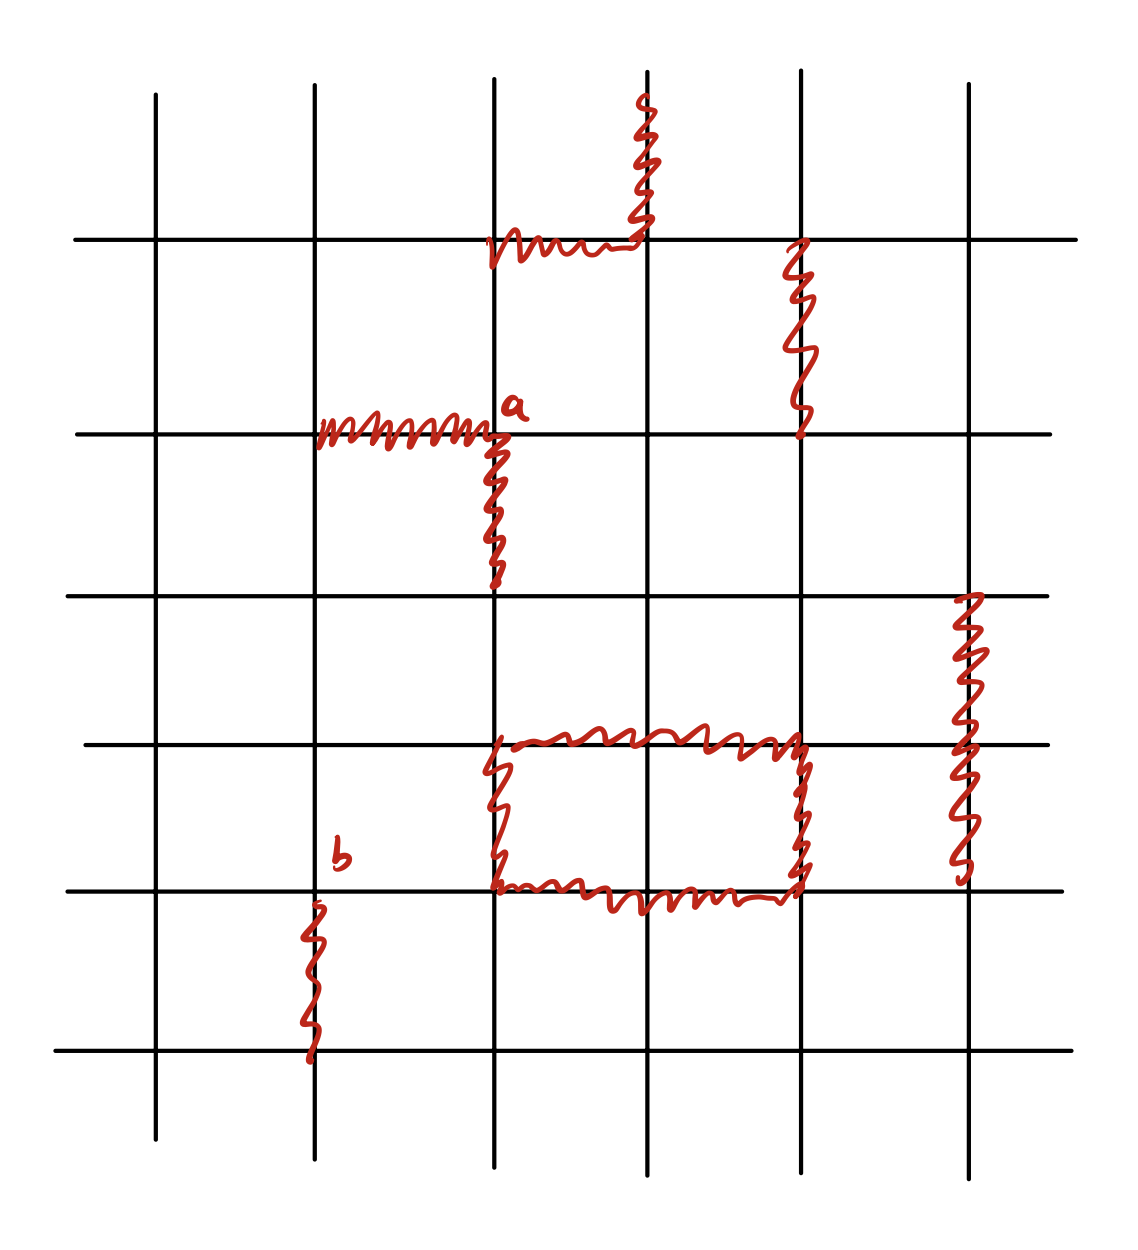
\includegraphics[scale=0.4]{Lectures/Images/lec1-strings.png}
\end{center}

With this point of view, let's figure out what the ground states look like in terms of the $X$-eigenstates. We want $a_s = 1$ for every star, thus $\prod_{j \in \text{star}(s)}X_j = 1$. This implies that the number of -1s in the product must be even. This means that the number of strings that touch a given site must be even. In the above picture, star($a$) obeys this condition while star($b$) does not. But, if $a_s = 1$ for every single star, this implies that the strings must form closed loops (else - at the endpoints of strings we end up with $a_1 = -1$). An allowed configuration is sketched below:

\begin{center}
    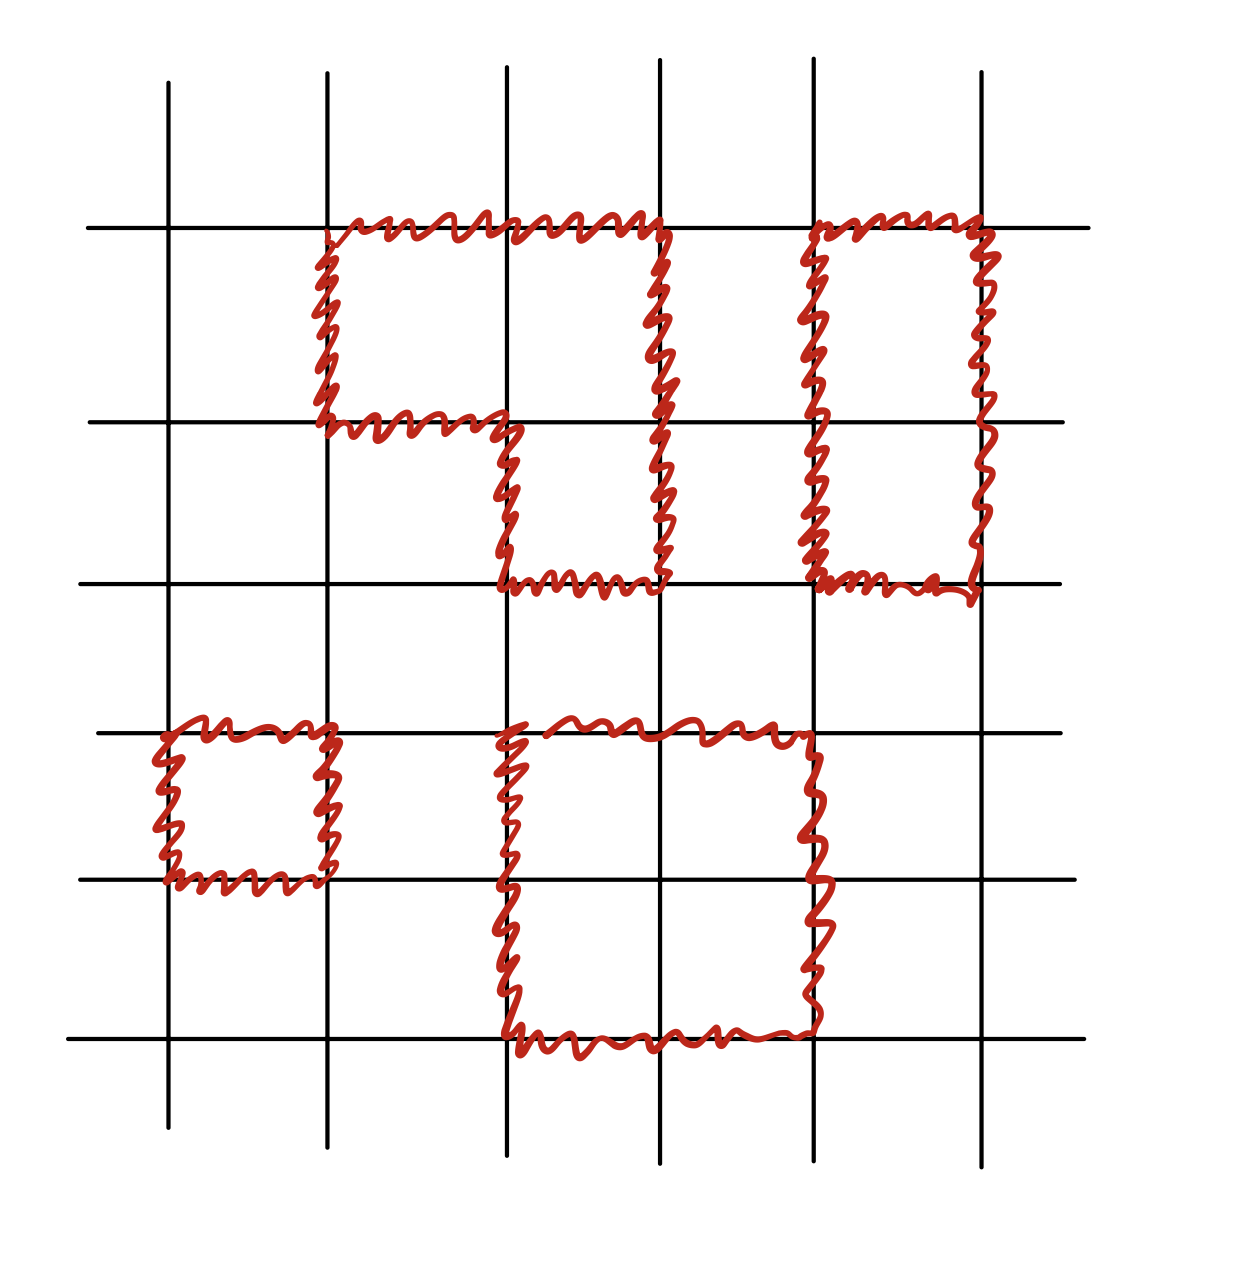
\includegraphics[scale=0.4]{Lectures/Images/lec1-stringsallowed.png}
\end{center}

Note that since $XZ = -ZX$, a given $B_p$ flips string occupation around a plaquette $p$, e.g.:

\begin{center}
    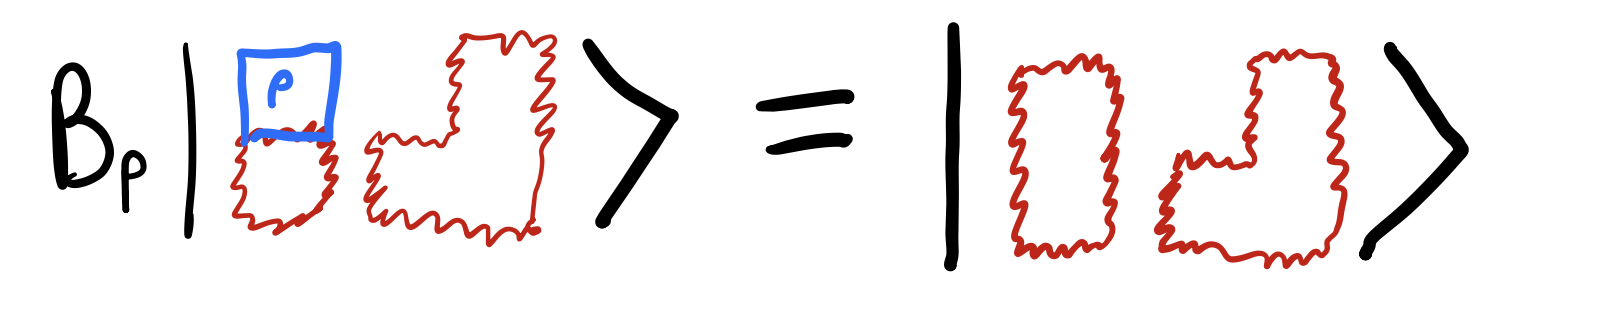
\includegraphics[scale=0.3]{Lectures/Images/lec1-plaquette.png}
\end{center}

But then all of the $a_s = b_p = 1$ requires that we have an equal amplitude superposition of all closed loop states (if this was not the case, the application of some $B_p$ would flip some loops and change the state - not an eigenstate!). Thus! There is a unique ground state:
\begin{equation}
    \ket{\Omega} = \ket{a_s = b_p = 1} = \sum_{\text{closed loop config $C$}}\ket{C}.
\end{equation}
We could draw an example $\ket{C}$ pictorially as:
\begin{center}
    
\includegraphics[scale=0.3]{Lectures/Images/lec1-closedloop.png}
\end{center}
It can be seen that $B_p$ only permutes the different $C$s to each other without changing their weight, so indeed the above is the $+1$ eigenstate of the $B_p$s. More formally, if $B_p\ket{\psi} = \ket{\psi}$ for all $p$, then:
\begin{equation}
    \braket{C}{\psi} = \bra{C}B_p\ket{\psi} = \braket{C'}{\psi}
\end{equation}
where $\ket{C'}$ is a different closed loop configuration. This implies that all of the amplitudes of the closed loop configurations have equal weight.

Note that formally there is an infinite number of closed loop configurations on an infinite plane, so there is a bit of a subtlety in normalizing the state (which requires the machinery of operator algebras, etc.) which we sweep under the rug.

Note that the above argument gave a unique state for $a_s = b_p = 1$, but for any choice of $\set{a_s, b_p}$ we can get a statement of a similar flavour. Thus, this justifies the choice of notation $\ket{\set{a_s, b_p}}$ as for a given choice of $a_s/b_p$ the state is unique.

Now, we have the full energy spectrum, as we have determined the degeneracy of all of the eigenspaces. We can thus determine the energy gap, which is the energy difference between the ground state and first excited state. Flipping one of the $a_s$ or the $b_p$ results in an energy penalty of $2$, and thus the energy gap is $\Delta = 2$. This is important because it means that we have a ``gapped Hamiltonian''. In comparison, there are ``gapless'' Hamiltonians for which the energy difference goes to zero in the thermodynamic limit. This distinction/property will be important when we discuss anyons - gapped Hamiltonians are the context in which they are currently understood.

\subsection{Excitations and String Operators}
There are two types of elementary excitations:
\begin{enumerate}
    \item $a_s = -1$ for some $s$; this is a ``charge'', and lives on a site.
    \item $b_p = -1$ for some $p$; this is a ``flux'', and lives on a plaquette.
\end{enumerate}
\begin{center}
    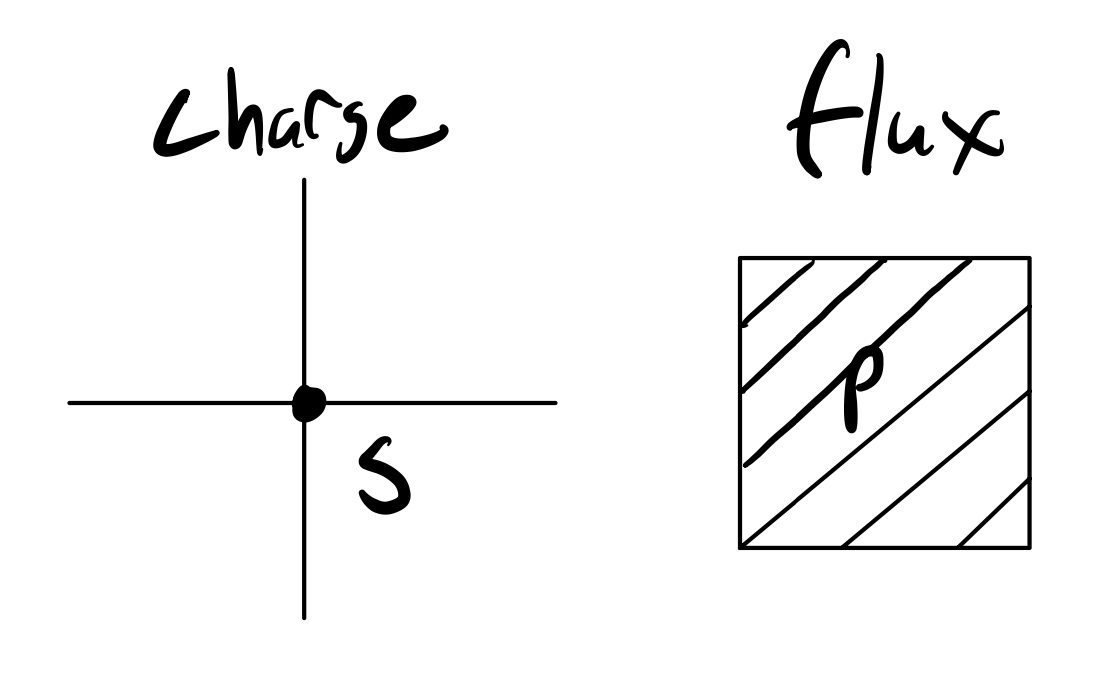
\includegraphics[scale=0.4]{Lectures/Images/lec1-excitations.png}
\end{center}
The terminology comes from $\ZZ_2$ gauge theory. We will see that these excitations are not conventional bosons or fermions that we may be familiar with.

If we visualize these excitations, adding a charge is like taking our superposition of all closed loops and then to each of those states adding one defect (with a string that goes off to infinity). Adding a plaquette takes the superposition of loops, and we count the number of loops that go around $p$ (a kind of winding number) and take that to be the sign of the configuration in the superposition. Pictorially, we have defects in the first case and vortices in the second.

Now, the question becomes how can we create charge or flux excitations? In spin systems you might be familiar with (e.g. creating a magnon in a Heisenberg spin chain) you would create them via a local operator. But here we actually apply a non-local string operator to create these excitations.

We define:
\begin{equation}
    W^Z(\gamma) = \prod_{j \in \gamma}Z_j
\end{equation}
where $\gamma$ is some open path on the lattice. The $W^Z(\gamma)$ is a string of $Z$s along $\gamma$. This string operator creates charge excitations at the two endpoints; notice that:
\begin{equation}
    [W^Z(\gamma), B_p] = 0
\end{equation}
this is obvious as the $B_p$s consist of $Z$s only. Less obvious is that the $W^Z(\gamma)$ commutes with almost all of the $A_s$ operators - all except at the endpoints of $\gamma$, $s_1$ and $s_2$. 

\begin{center}
    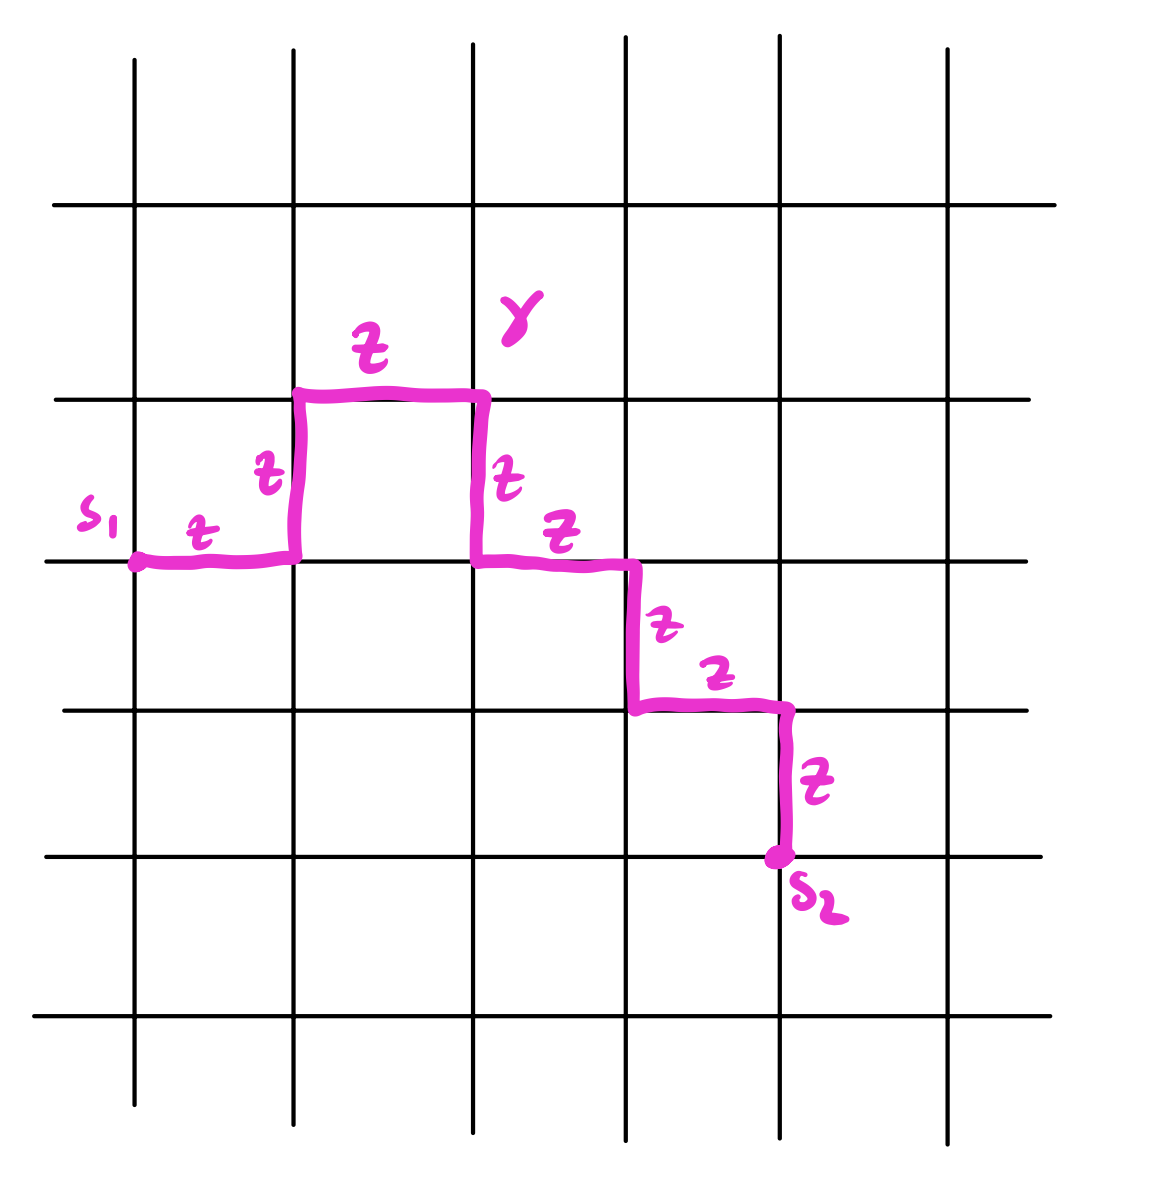
\includegraphics[scale=0.4]{Lectures/Images/lec1-stringop.png}
\end{center}

Let us argue this. At intermediate points along the path each of the points have an even number of strings so we have commutation. At the endpoints, we only have 1 link and so we have anticommutation:
\begin{equation}
    W^Z(\gamma)A_{s_{1,2}}  = -A_{s_{1,2}}W^z(\gamma)
\end{equation}
What are the implications of this? Looking at the ground state $\ket{\Omega} = \ket{\set{a_s=b_p=1}}$:
\begin{equation}
    W^Z(\gamma)\ket{\Omega} = \ket{\set{a_{s_1} = a_{s_2} = -1, \text{others} = 1}}.
\end{equation}
and we can see this because the string operator only flips the stars at the endpoints, and commutes with everything else. Thus, we conclude that the $W^Z(\gamma)$ creates charges at the two endpoints of $\gamma$, as claimed.

An important observation with regard to string operators; If $\gamma'$ is a different path with the same endpoints, then the string operator $W^z(\gamma')$ applied to the ground state yields the \emph{exact} same state (even up to the same phase):
\begin{equation}
    W^Z(\gamma)\ket{\Omega} = W^z(\gamma')\ket{\Omega}
\end{equation}
this is the notion in which string operators are ``flexible''. To see this, note that $W^Z(\gamma') = W^Z(\gamma)\prod_{p \in \text{int}(\gamma' \cup \gamma)}B_p$, i.e. the two operators are related via a product of plaquette operators in the interior of the two paths. Thus:
\begin{equation}
    W^Z(\gamma')\ket{\Omega} = W^z(\gamma)\prod_{p \in \text{int}(\gamma' \cup \gamma)}B_p\ket{\Omega} = W^Z(\gamma)\ket{\Omega}
\end{equation}
where we have used that $\ket{\Omega}$ is the $+1$-eigenstate of all the $B_p$s.

\begin{center}
    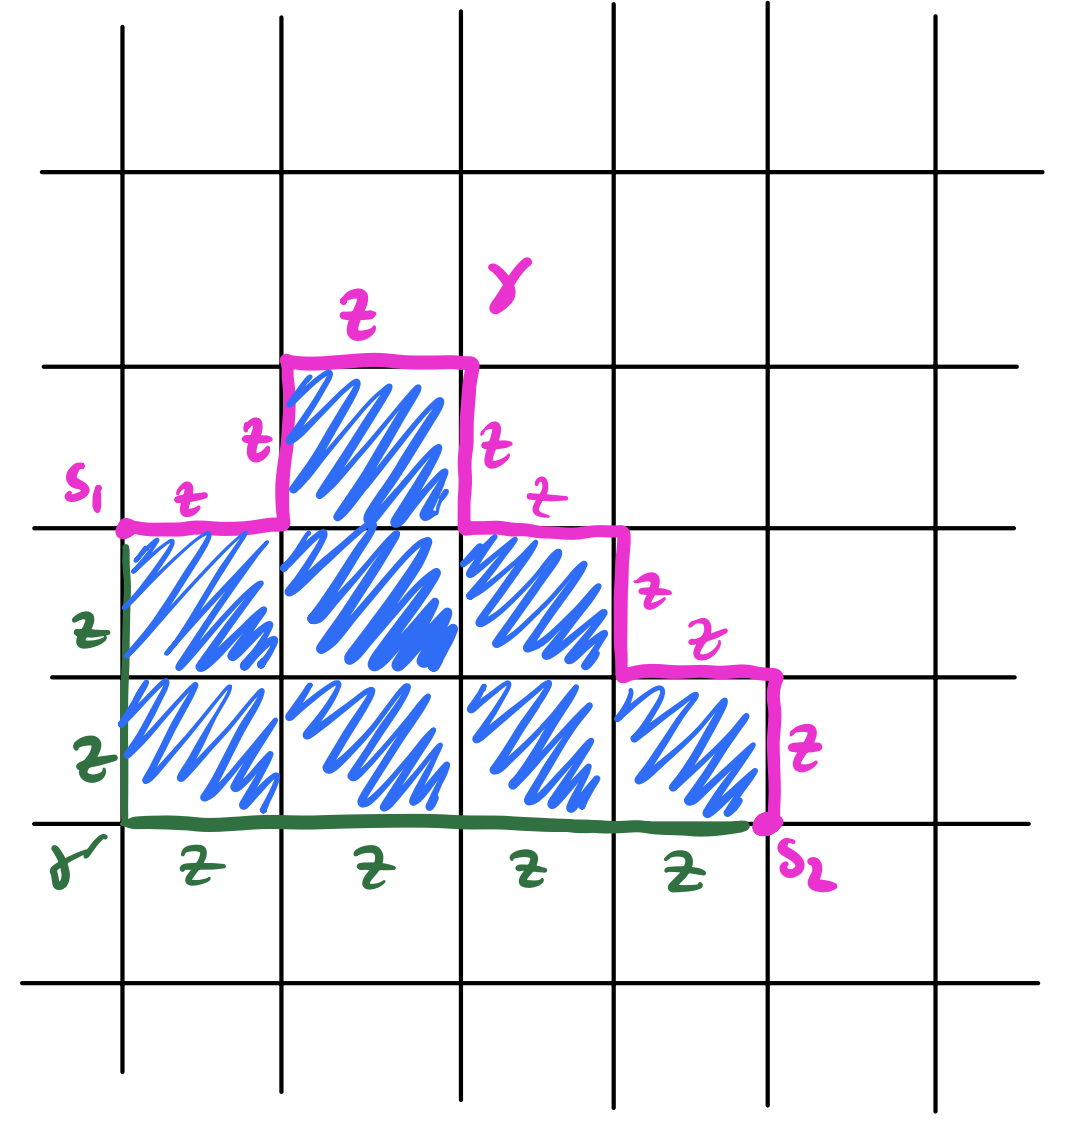
\includegraphics[scale=0.4]{Lectures/Images/lec1-flexible.png}
\end{center}

Relatedly, if $\gamma$ is a closed loop then:
\begin{equation}
    W^Z(\gamma)\ket{\Omega} = \ket{\Omega}
\end{equation}
which follows from the fact that a closed loop is just a product of $B_p$s.

\begin{center}
    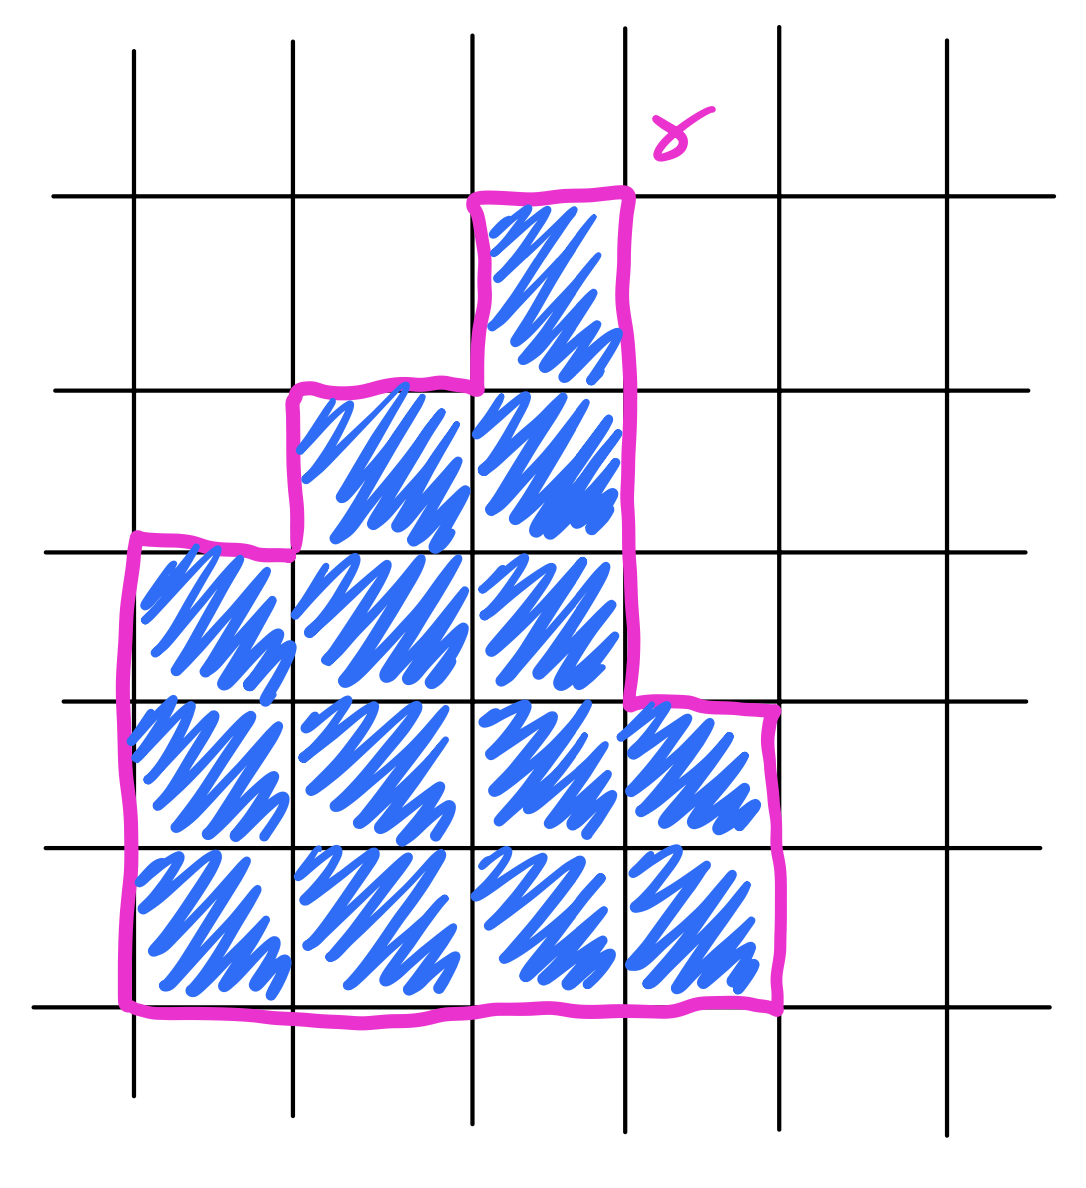
\includegraphics[scale=0.4]{Lectures/Images/lec1-loopstringop.png}
\end{center}


These features - which currently seem pretty specific to the toric code model - are in fact quite general. Any system with anyons have string operators with these properties!

A last comment to provide some physical intuition for what the string operator is. We can view it as the physical process of first creating two charges (by applying a single $Z$), then moving that charge via the application of further $Z$s along the path. I.e. a string operator is just creating two charges and separating them. This makes the notion that the string is flexible intuitive; we should get the same state (up to some phase) if the particles are created and end up in some separated location(s), no matter how we move them there.

\end{document}